\section{Algebraic evidence-cost maps}
\label{app:post-maps}

The 216 fixed-overlap and 216 declining-overlap configurations evaluate the
full 49-point threshold grid using only design inputs. They retain subgroup
mass, exact exposure, legal residual moments and the available coloring count.
These are procedure-specific sufficient radii and contain no sampled outcomes;
they do not verify a minimax rate or a necessary evidence requirement.

\begin{figure}[ht]
\centering
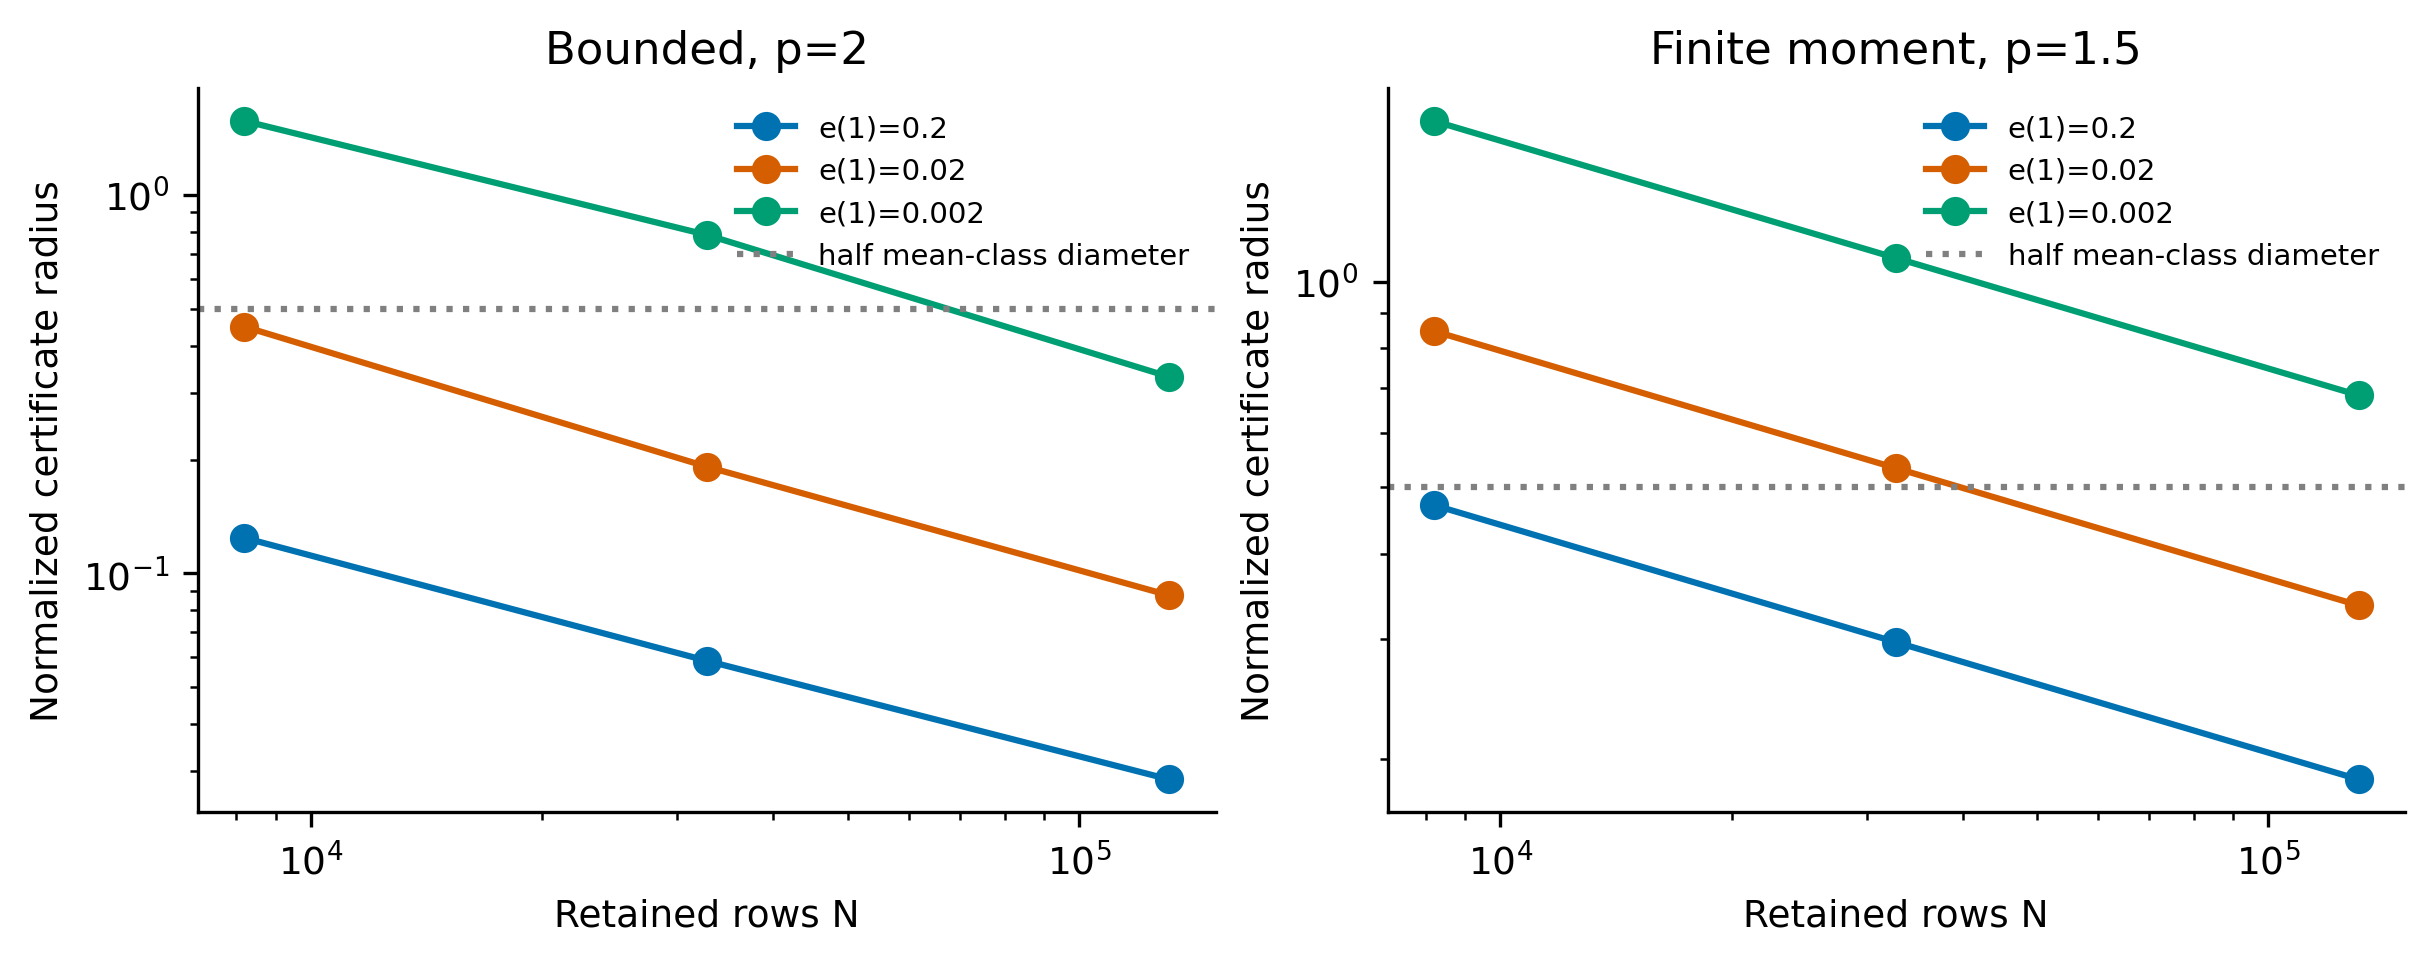
\includegraphics[width=\linewidth]{figures/design_v1/analytic_evidence_cost.png}
\caption{Deterministic normalized certificate radii at subgroup mass near .1,
available coloring count 2, family size 16 and total failure budget .05.
The bounded panel permits a design-only choice among truncation, Hoeffding
and Bernstein. The finite-moment panel uses the declared Pareto-source
residual envelope. No Monte Carlo error bars apply.}
\label{fig:post-cost}
\end{figure}

\begin{figure}[ht]
\centering
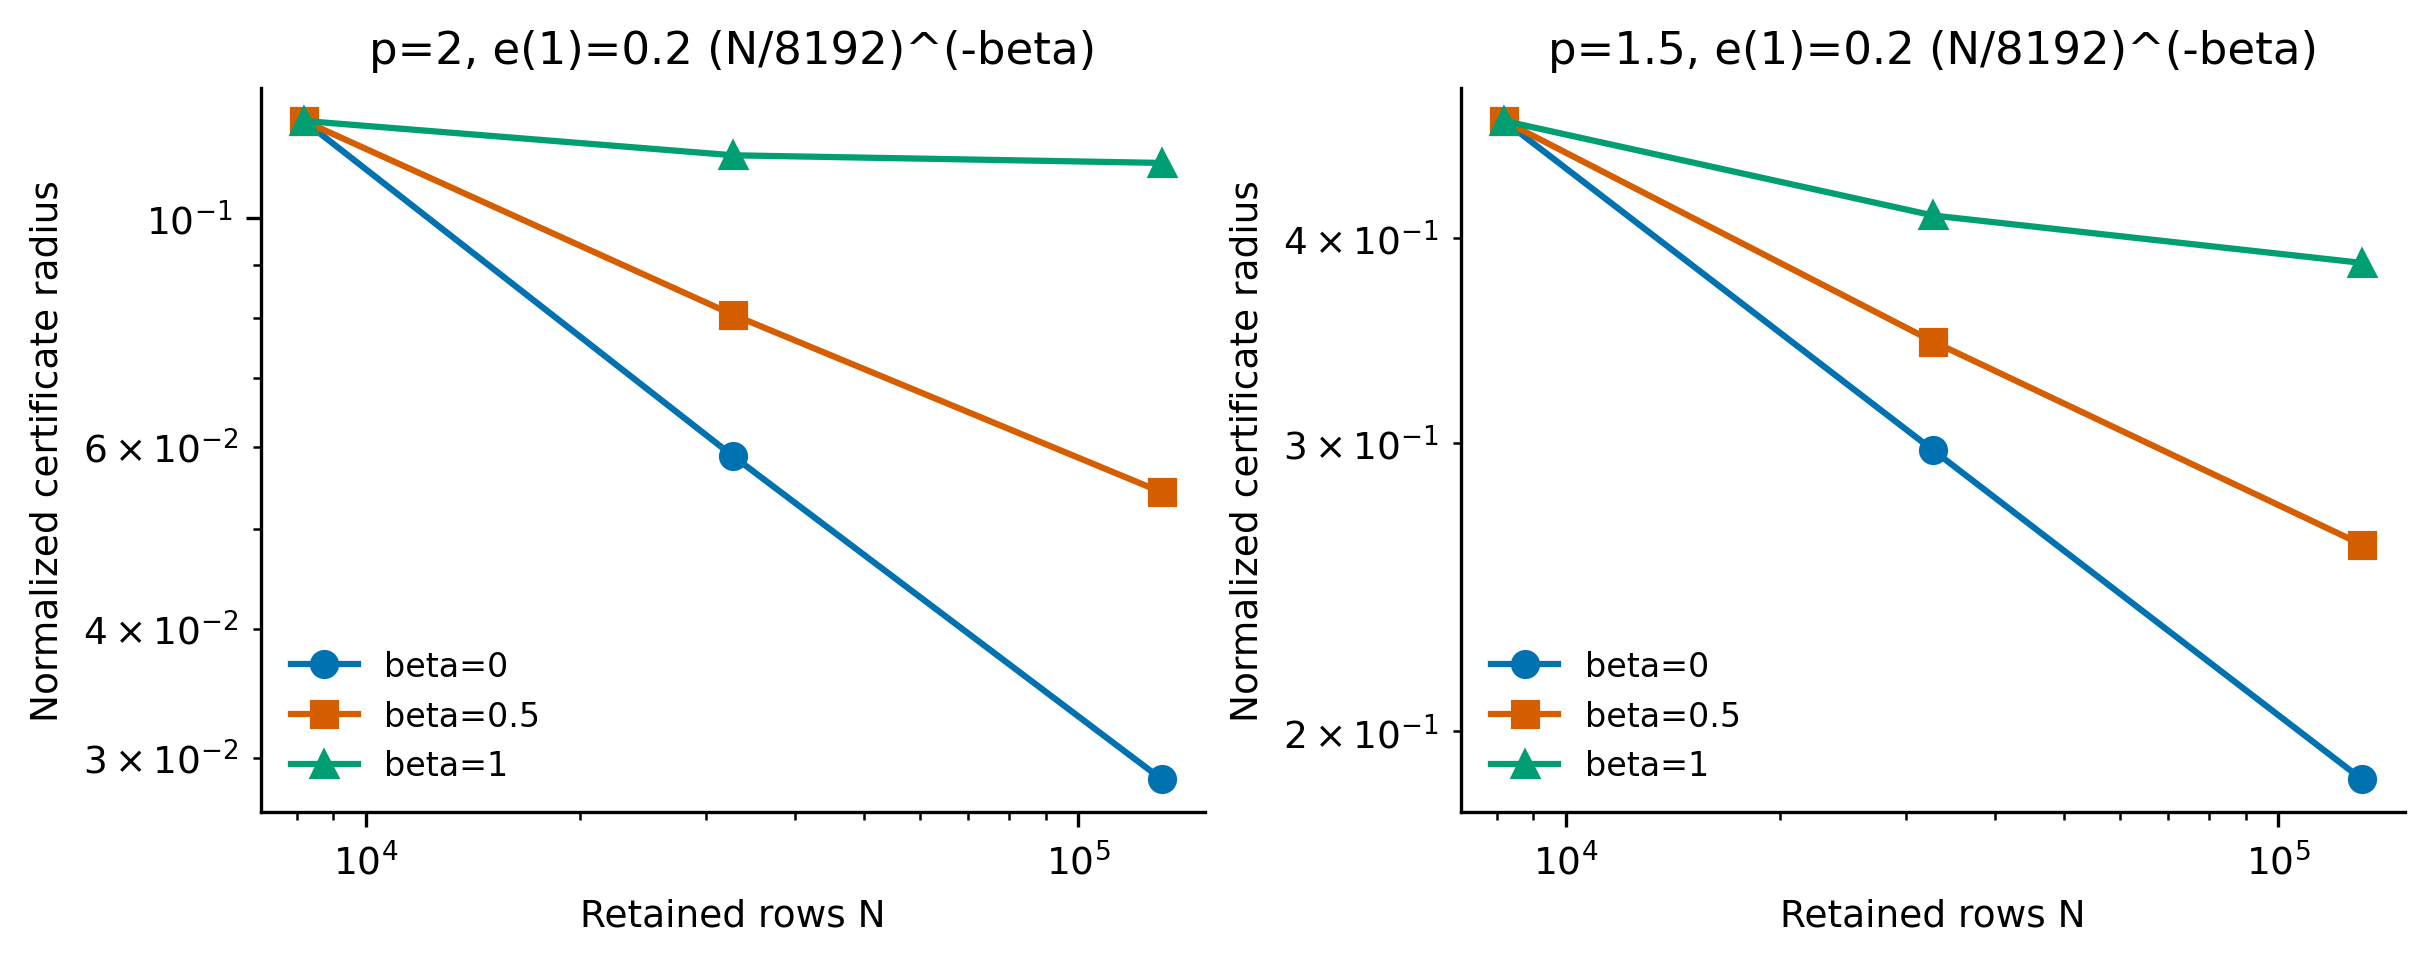
\includegraphics[width=\linewidth]{figures/design_v1/analytic_declining_overlap.png}
\caption{Declining exposure can offset growing row count. The design-only
schedule is $\epsilon_N=.2(N/8192)^{-\beta}$, with the other quantities as in
Figure~\ref{fig:post-cost}. These are procedure-specific sufficient radii,
not a sharp necessary cost or an empirical result for arbitrary weak overlap.}
\label{fig:post-declining}
\end{figure}
